\chapter{Introduction}
The flow around circular cylinders has become an important research field. In recent years, this kind of problems are increasingly appearing in biology, medical science, and chemistry, waiting for people's further research.


\section{Flow Around Circular Cylinders}
The flow past a bluff body is of importance in both the nature and engineering practice. Ships run on the surface of water, aircrafts navigate the air, the river flows through the bridge, the sea around the island, and the wind blows over tall buildings. These are all the examples of the flow past a bluff body, which can be observed in every corner of the world, and are closely linked with our life.

Flow around circular cylinders is an classical problem in fluid mechanics. The flow state can be divided into several stage\cite{Zdravkovich1997b}. In domain far from the cylinder, the flow can be described with potential flow theory. In domain near the cylinder, the flow can be divided into four parts, as shown in Figure \ref{fig: flow area}\cite{demartino2017aerodynamics}. This four regions are retarded flow, boundary layer, sidewise region, and wake. When fluid flow across a plate, boundary layer forms from the leading edge of the plate. The original fluid state is laminar, but the laminar flow state transfers to turbulent as the fluid moves downstream. With the increase of Reynolds number, the transition zone moves upstream. In the same way, when fluid flow around a cylinder, the transition of fluid state also moves upstream, and the transition point passes through four districts. Relevant flow state are called transition in wake (TrW), transition in shear layer (TrSL), and transition in boundary layer (TrBL).

\begin{figure}
	\centering
	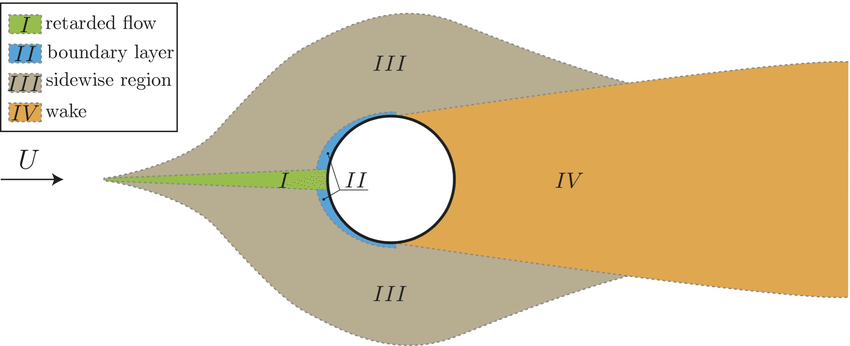
\includegraphics[scale=.4]{figs/Regions-of-disturbed-flow-around-a-perfect-circular-cylinder}
	\caption{The division of the flow area\cite{demartino2017aerodynamics}.}
	\label{fig: flow area}
\end{figure}

Laminar state (L). When 0 < $Re$ < 4--5, the fluid flows around the outline of the cylinder, and the streamlines are bilaterally symmetrical. When 4--5 < $Re$ < 30--48, the fluid begins to separate from the surface of the cylinder. A closed attachment vortex appears at the back of the cylinder, but does not shed from the surface of the cylinder. The fluid is in steady state now. When 30--48 < $Re$ < 180--200, the vortexes on the surface of the cylinder shed and flutter from the close t the distance slowly. During the laminar state, $Re$ > 30--48, the wake transitions from the steady to unsteady state, and the tail end of streamlines begins wiggling, with a sinusoidal movement. Then during $Re$ > 45--65, shear layer rolls up a set of wave crests and hollows. Then arise a list of vortexes, which are so called vortex street. 

Transition in the wake (TrW). When 180--200 < $Re$ < 220--250, fluid state's transition from laminar to turbulent occurs in the wake far away from the cylinder (transition of eddies in the wake, TrW1). With the increase of Reynolds number, the transition point moves upstream. When 220--250 < $Re$ < 350--400, the transition occurs near the cylinder (transition of irregular eddies during its formation, TrW2). Eventually, the fluid is in turbulent state upon vortexes' generation. An important phenomenon between TrW1 and TrW2 is that the laminar wake instability mode of formation and shedding is replaced by the turbulent eddy roll up and shedding mode from the cylinder\cite{Zdravkovich1997b}.

Transition in the shear layer (TrSL). The state is subcritical. When 350--400 < $Re$ < 1k--2k, ? 

Transition in boundary layer (TrBL). The state is called critical state. When 100k--200k < $Re$ < 300k--340k, ?

Turbulent state (T). With the increase of Reynolds number, the whole flow field become turbulent state.


\section{Flow Through Porous Medium}
Flow through porous media is a common phenomenon in many branches of engineering and science, such as ground water hydrology, reservoir engineering, soil science, soil mechanics and chemical engineering\cite{Bear2013}. Aquifers in ground water hydrology, oil reservoirs (shown in Figure \ref{fig: Aquifers and oil reservoirs}), soil, porous or fissured rocks, ceramics, filter paper, sand filters, and a loaf of bread are all the examples of flow through porous medium. In addition, fluidized bed, biological filtration, rainfall, microcarries and scaffold, biological chemical filters, and porous heat exchange are also important research field.

\begin{figure}
	\centering
	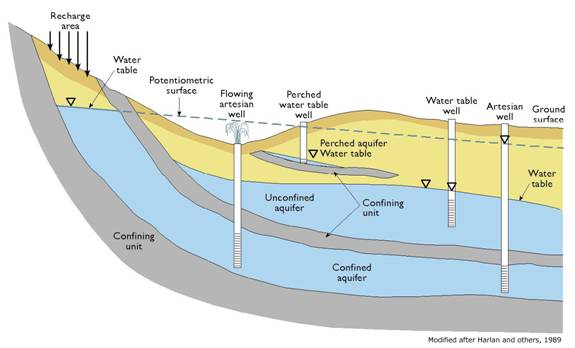
\includegraphics[height=.2\textheight]{figs/Aquifers}
	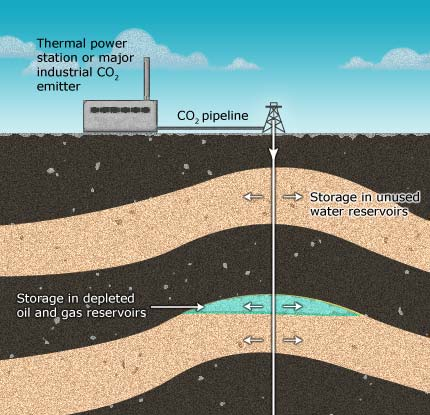
\includegraphics[height=.2\textheight]{figs/Oil-reservoirs}
	\caption{Aquifers and oil reservoirs}
	(Resource: Colorado Geological Society; Alan Sherwood and Jock Phillips, 'Coal and coal mining - The future of coal', Te Ara - the Encyclopedia of New Zealand)
	\label{fig: Aquifers and oil reservoirs}
\end{figure}

Porous medium can be simply described as "a solid with holes". From the perspective of fluid, it is a portion of space occupied by heterogenous or multiphase matter; the solid phase should be distributed throughout the porous medium within the domain occupied by a porous medium; at least some of the pores comprising the void space should be interconnected\cite{Bear2013}.

The continuum approach to pure fluid transfers the description of fluid from molecular level or viewpoint to fluid continuum, which is microscope level. In the similar way, the continuum approach to porous media can be introduced, in order that we can transfer the description of porous medium from microscopic level to representative volumetric element (REV), which is macroscopic level. It is still a continuum approach, but on a higher level. As a result, porous medium can be described in this way, and mass and momentum equations can be established.


\section{Flow past and Through Porous Bluff Bodies}


\section{Research Question and Dissertation Structure Arrangement}
